\section{Difference Image Analysis: Solar System Objects}
\label{sec:dia_solar_system}

\subsection{Difference Image Association}
\label{sec:dia_solar_system_assoc}

So far, difference images have been made only of two fields very far from the ecliptic, where solar system objects are very rare. Known-object association ran, but (correctly) associated no difference image sources to known objects. 

\subsection{Difference Image Linking}
\label{sec:dia_solar_system_link}

We tested tracklet creation with {\tt make\_tracklets}, the first stage of {\em unknown} asteroid discovery for LSST, on the two available sets of difference images, though asteroids were unlikely to be found in these regions of the sky. The first field included 10 visits with on average 840 sources per visit, while the second had 12 visits with on average 430 sources. These numbers are encouragingly low, indicating that Rubin difference images are fairly clean. For this test case, we set {\tt make\_tracklets} to require a minimum of 5 sources per tracklet, but it produced only 9 total tracklets, all with fewer than 5 detections, inconsistent photometry, and relatively high Great Circle residual (GCR)\footnote{Defined only for tracklets with more than two points, the GCR is the RMS residual relative to the best-fit trajectory that follows a Great Circle on the sky at constant angular velocity. Real asteroids, unless they are very near the Earth, produce tracklets with very low intrinsic GCR: hence, elevated GCR usually indicates a spurious tracklet.}. Manual examination of image cutouts confirmed that the tracklets were entirely composed of spurious sources.

More interesting is the nature of the spurious sources that made up the tracklets. All were associated with bright stars, including diffraction rays, incompletely subtracted scattered light halos, and subtraction residuals near the PSF core. This is very good news, as all of these types of spurious detections can be eliminated through pre-screening of the source catalogs. 

Early data suggests that LSST will produce fairly clean difference image source catalogs for the asteroid discovery pipeline and that pre-screening can make them even cleaner. This is important, because simulations indicate the LSST specifications for the minimum discoverable asteroid (six detections, making up three two-point tracklets, within a two-week time span) are on the edge of what is statistically possible without an unacceptable false positive rate. Hence, it is vitally important for the difference image source catalogs to be as clean as possible. There's a lot of work to do, but the early indications have us cautiously optimistic.

\section{Single-epoch Image Analysis: Solar System Objects}
\label{sec:sia_solar_system}

\subsection{Single-epoch Association}
\label{sec:association}



Ten images taken in one field on 2024-11-06 and ten each in four fields on 2024-11-23 were close enough to the ecliptic for possible asteroid association. Across the five fields, we associated 828 sources with known asteroids, including 128 unique objects. The 24 objects associated on 2024-11-06 are shown in Figure \ref{fig:solar_system_positions}. We compared the sources' astrometry to our ephemerides, as shown in Figure \ref{fig:solar_system_residuals}. We find very low bias: the median unsigned error is 13 mas, indicating that there are no major errors in either timing or astrometry. We also find low variance, with standard deviationsin RA and Dec of 41 and 44 mas respectively, though in an especially bright and therefore low-variance sample of known objects. Evaluating the precision of asteroid association tests the whole software chain, including the astrometry pipeline, ephemerides computation, and image timing. In sum, the total error contributed by these different systems appears to be low enough for high-confidence association of known asteroids.

\begin{figure}
  \label{fig:solar_system_positions}
  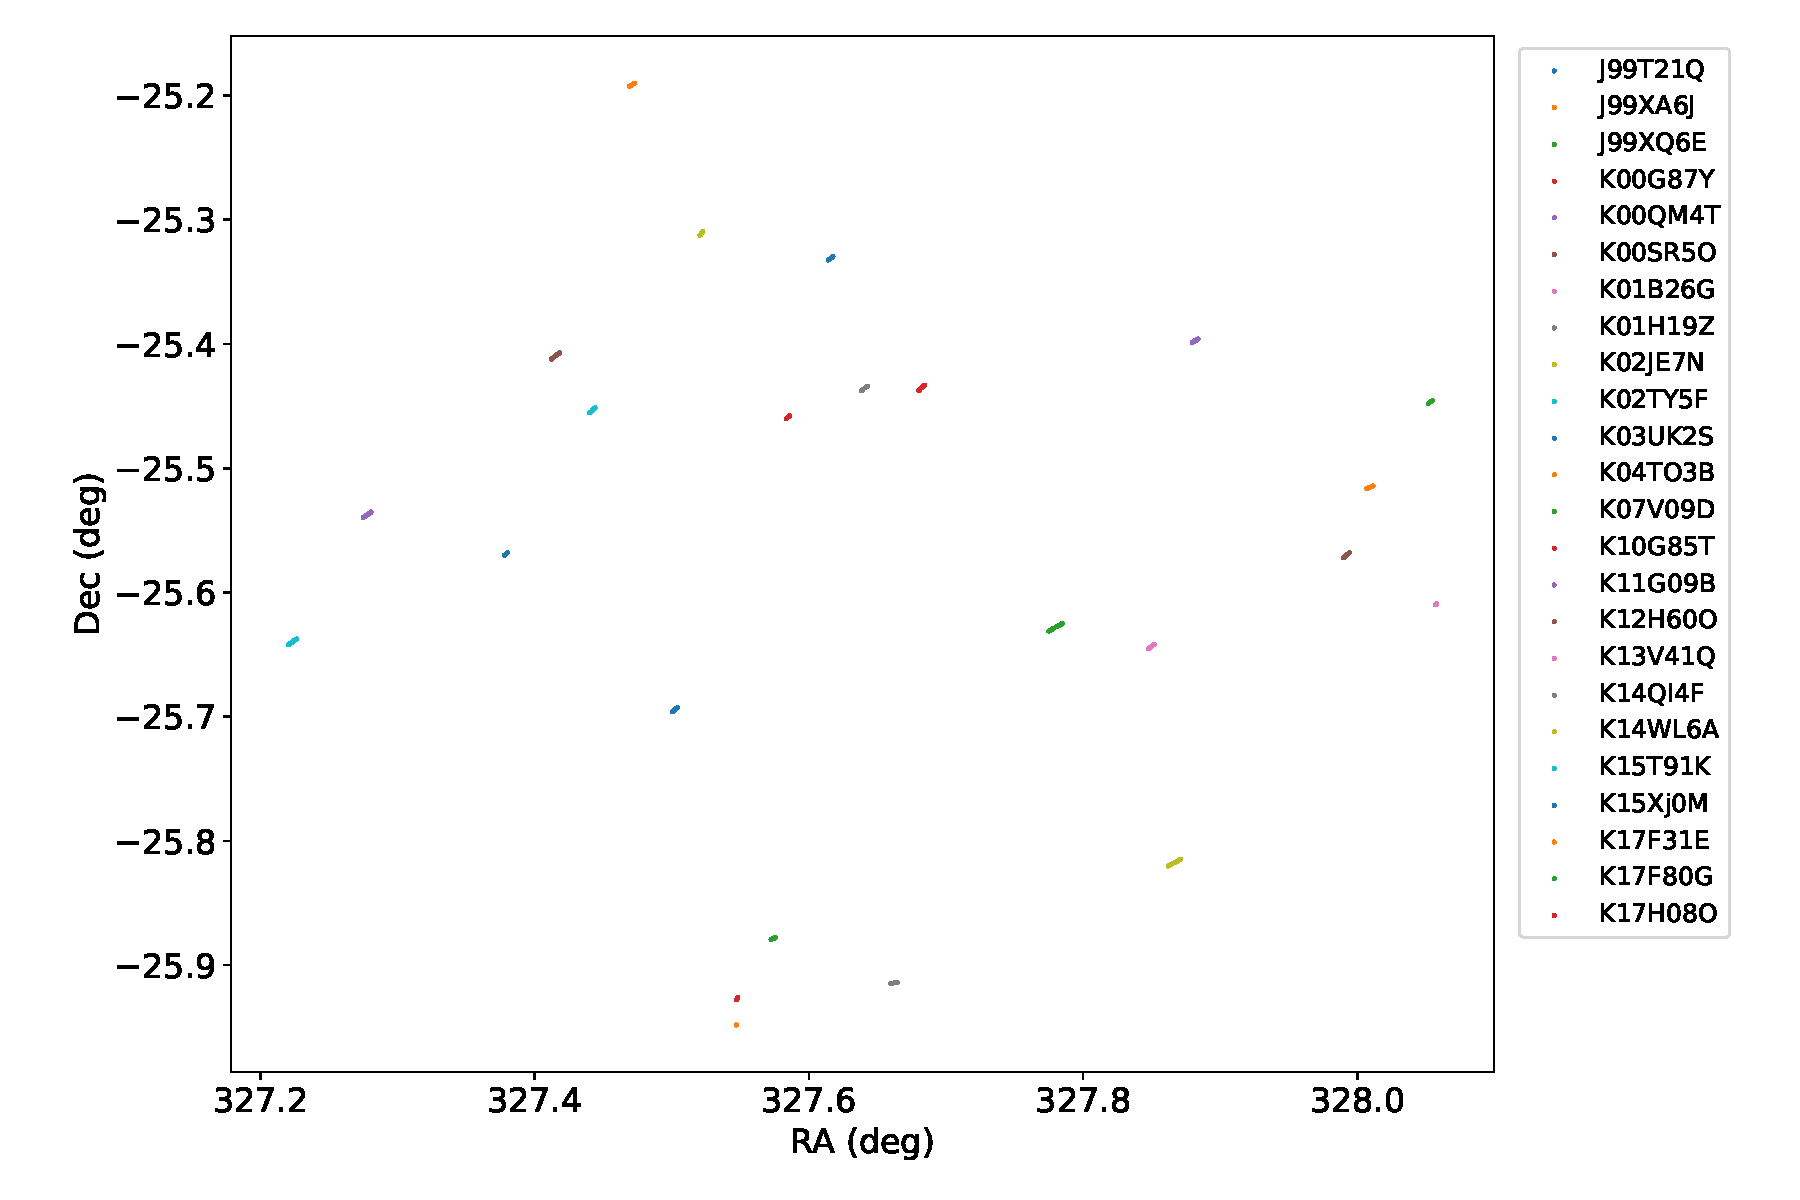
\includegraphics[width=\textwidth]{sso_figures/24_asteroids.pdf}
  \caption{Positions of the 24 asteroids associated in images from 2024-11-06.}
\end{figure}

\begin{figure}
  \label{fig:solar_system_residuals}
  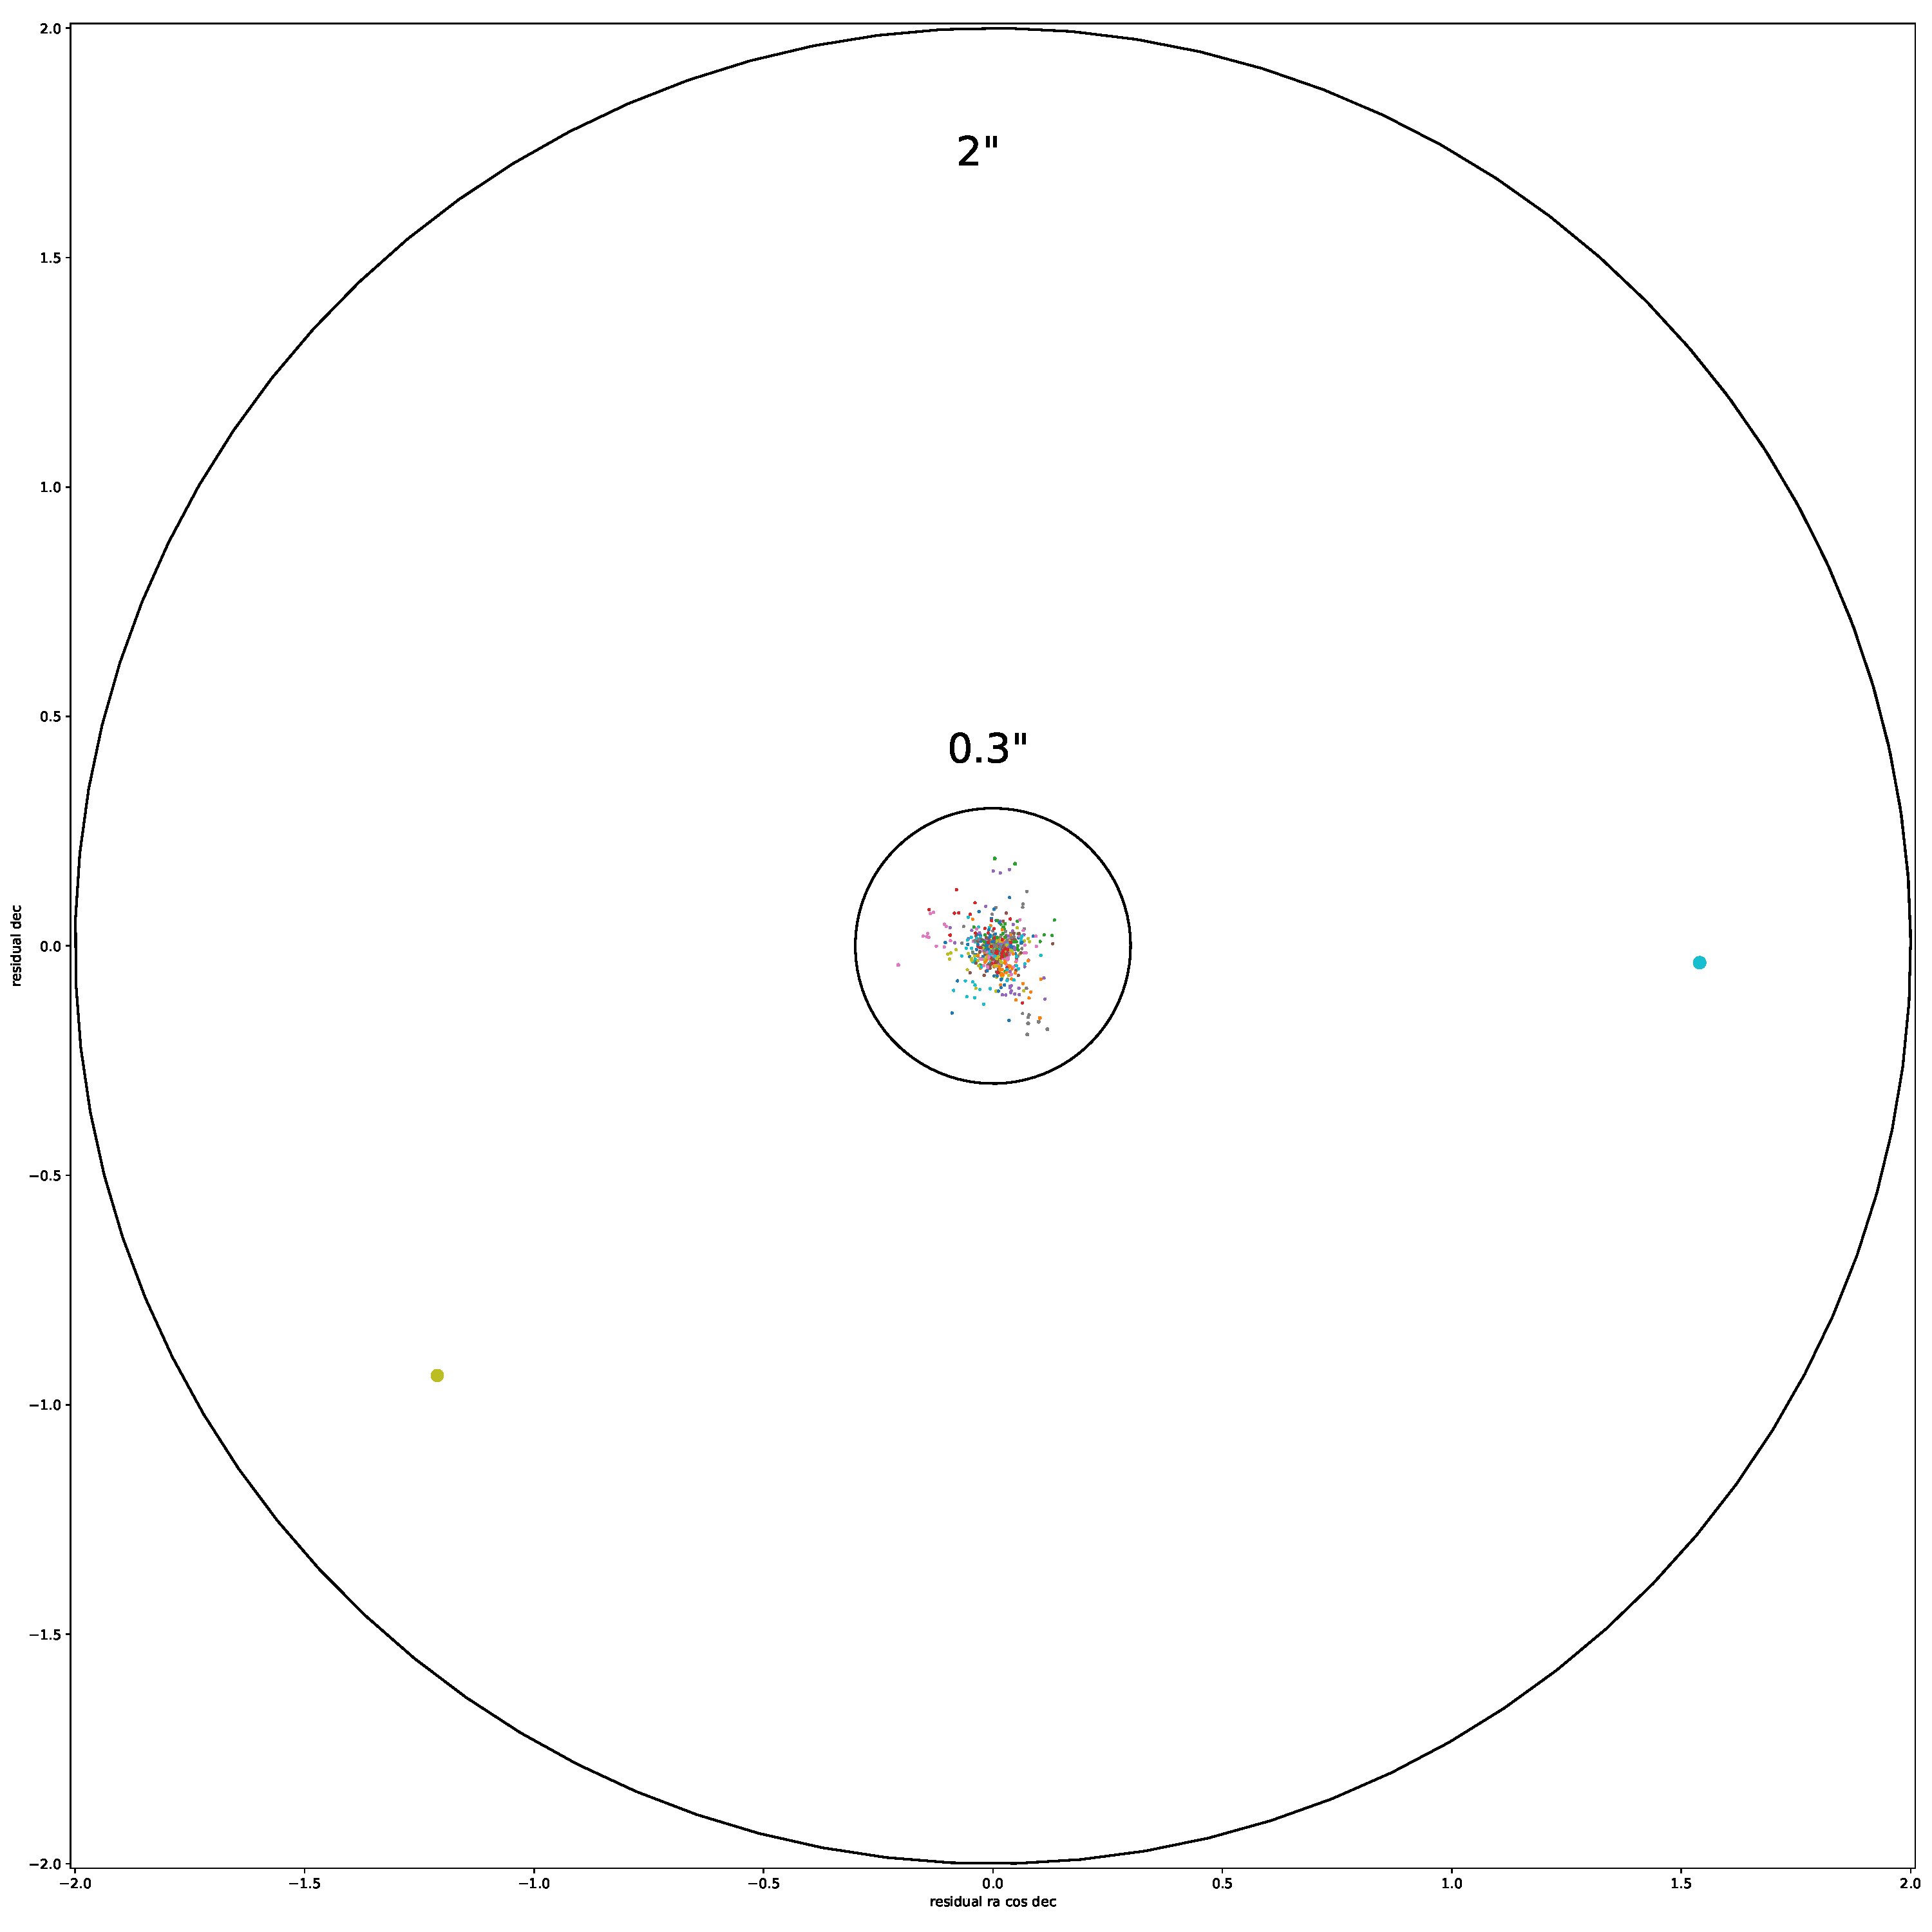
\includegraphics[width=\textwidth]{sso_figures/sso_residuals.pdf}
  \caption{Astrometric residuals of the 633 sources associated to 104 asteroids on 2024-11-23. All but two sources have residuals under 0.3 arcseconds, while the two outliers have been identified by visual inspection as mis-associations of undetected asteroids.}
\end{figure}

\subsection{Single-epoch Linking}
\label{sec:linking}

We attempted to link asteroids in single-epoch source catalogs including the fields in section \ref{sec:association} relatively near the ecliptic. In contrast to the difference images averaging 430-840 sources per visit, single-epoch images contained 11,000-23,000 sources per visit, mostly stars. The first reasonable test involved ten images taken on November 6. From an average of 16,000 sources per visit, {\tt make\_tracklets} found 3,068 tracklets with at least five points. While most of these were unquestionably spurious, nine of them were ten-point tracklets (i.e. detected in {\em every one} of the ten visits), showed excellent photometric consistency, and relatively low GCR: very likely real asteroids.

We selected the ten-point tracklet with the very lowest GCR (0.046 arcsec) and checked it against known asteroid ephemerides, obtaining a match to the main belt asteroid \textbf{(193300) 2000 SO275}, a 20th magnitude object with a very well-constrained orbit. \textbf{(193300) 2000 SO275} was the {\em very first asteroid confirmed to have been detected with the Simonyi Survey Telescope.} We evaluated LSST's astrometric precision by comparing these detections to predicted positions from JPL. The RMS astrometric offset was found to be 29 milli-arcseconds (mas), with a systematic bias (the median observed-calculated residual) of only 14 mas in RA and 3 mas in Dec. These errors are statistically consistent with zero, as expected. We also probed for timing errors, which would produce a positional offset in the direction of motion. Dividing the along-track component of the astrometric offsets by the measured angular velocity, we found a median time offset of 0.3 seconds --- consistent with zero at the 0.5$\sigma$ level.

All of the other ten-point tracklets were found to correspond to known asteroids, as did 12 additional tracklets with 7--9 points, consistent photometry, and relatively low GCR. In total, 21 real asteroids were found by {\tt make\_tracklets} in this single field, demonstrating its ability to discover asteroids in LSST catalogs.
